\documentclass[11pt]{article}

\usepackage{graphicx}
\usepackage{hyperref}
\usepackage{longtable}
\usepackage{geometry}
\usepackage{tikz}
\usetikzlibrary{arrows.meta,positioning,shapes.geometric}

\geometry{margin=1in}

\title{Standard Operating Procedure (SOP)\\
Simulation of SARS-CoV-2 Wastewater Sequencing Samples}
\author{Dieter Best (dieter.best@cdph.ca.gov)}
\date{\today}

\begin{document}

\maketitle

\section{Purpose}

This document describes a workflow used to simulate SARS-CoV-2 wastewater sequencing samples.  
The pipeline generates synthetic sequencing reads representing mixtures of viral strains and includes realistic sequencing artifacts such as RNA fragmentation and primer dropout.

The resulting datasets are used for benchmarking bioinformatics pipelines for viral surveillance, variant detection, and strain deconvolution.

\section{Pipeline Flow Diagram}

The following diagram shows the overall data processing flow of the pipeline.

\begin{center}
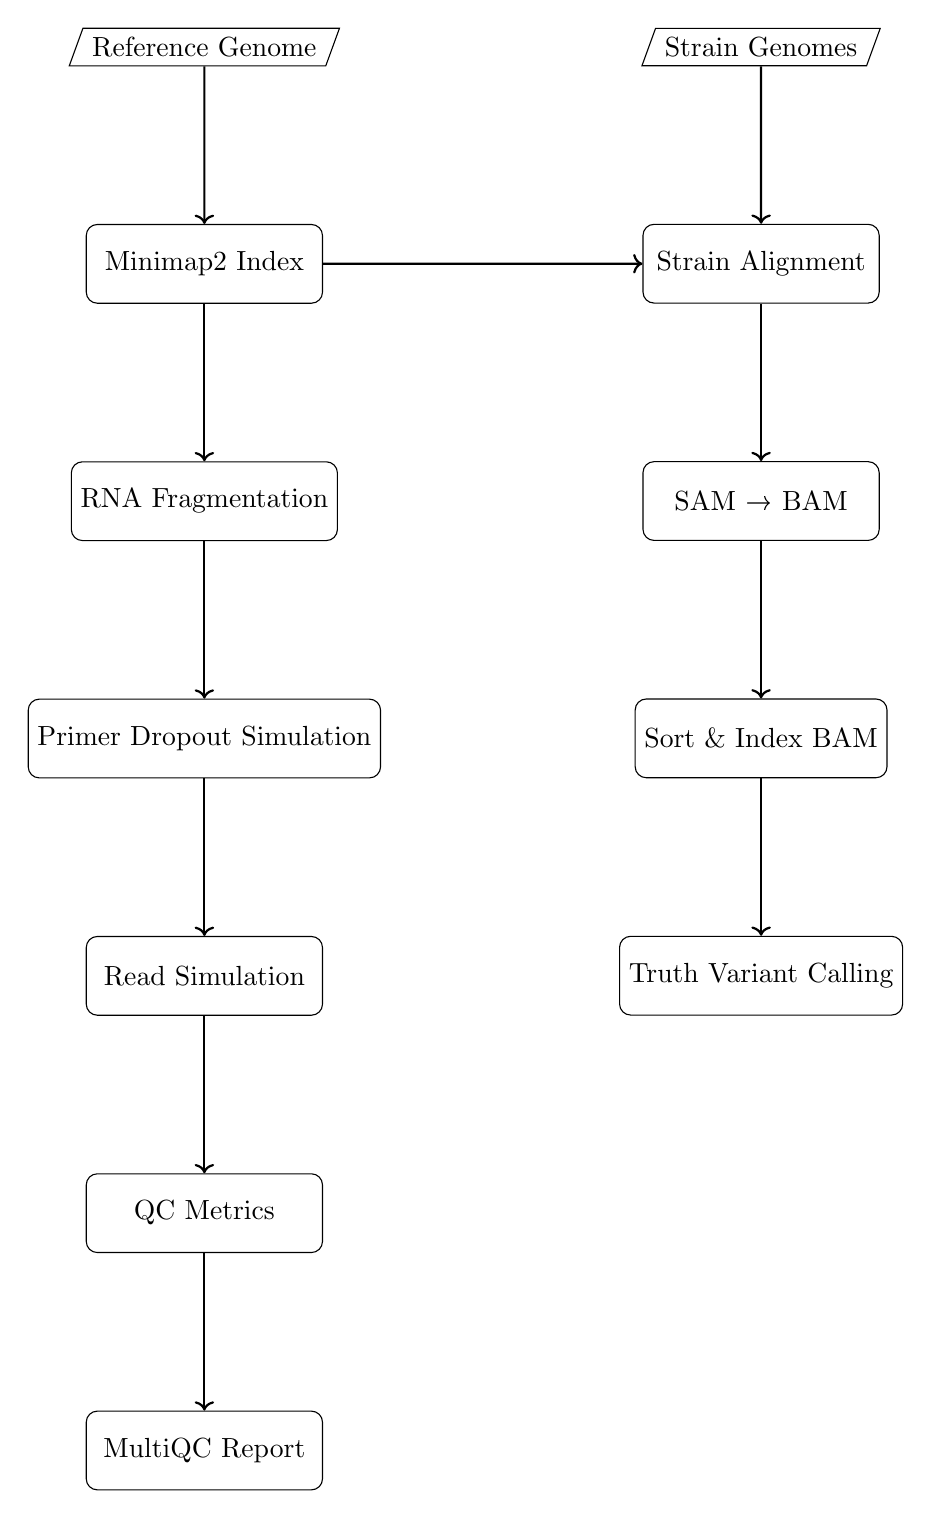
\begin{tikzpicture}[
node distance=2cm,
process/.style={rectangle, draw, rounded corners, minimum width=3cm, minimum height=1cm},
data/.style={trapezium, trapezium left angle=70, trapezium right angle=110, draw},
arrow/.style={->, thick}
]

\node[data] (ref) {Reference Genome};
\node[data, right=4cm of ref] (strain) {Strain Genomes};

\node[process, below=of ref] (index) {Minimap2 Index};

\node[process, below=of strain] (align) {Strain Alignment};

\node[process, below=of align] (bam) {SAM → BAM};

\node[process, below=of bam] (sort) {Sort \& Index BAM};

\node[process, below=of sort] (vcf) {Truth Variant Calling};

\node[process, below=of index] (fragment) {RNA Fragmentation};

\node[process, below=of fragment] (dropout) {Primer Dropout Simulation};

\node[process, below=of dropout] (reads) {Read Simulation};

\node[process, below=of reads] (qc) {QC Metrics};

\node[process, below=of qc] (multiqc) {MultiQC Report};

\draw[arrow] (ref) -- (index);
\draw[arrow] (strain) -- (align);
\draw[arrow] (index) -- (align);
\draw[arrow] (align) -- (bam);
\draw[arrow] (bam) -- (sort);
\draw[arrow] (sort) -- (vcf);
\draw[arrow] (index) -- (fragment);
\draw[arrow] (fragment) -- (dropout);
\draw[arrow] (dropout) -- (reads);
\draw[arrow] (reads) -- (qc);
\draw[arrow] (qc) -- (multiqc);

\end{tikzpicture}
\end{center}

\section{Workflow Architecture Diagram}

The workflow uses hierarchical parallelization with WDL scatter blocks.

\begin{center}
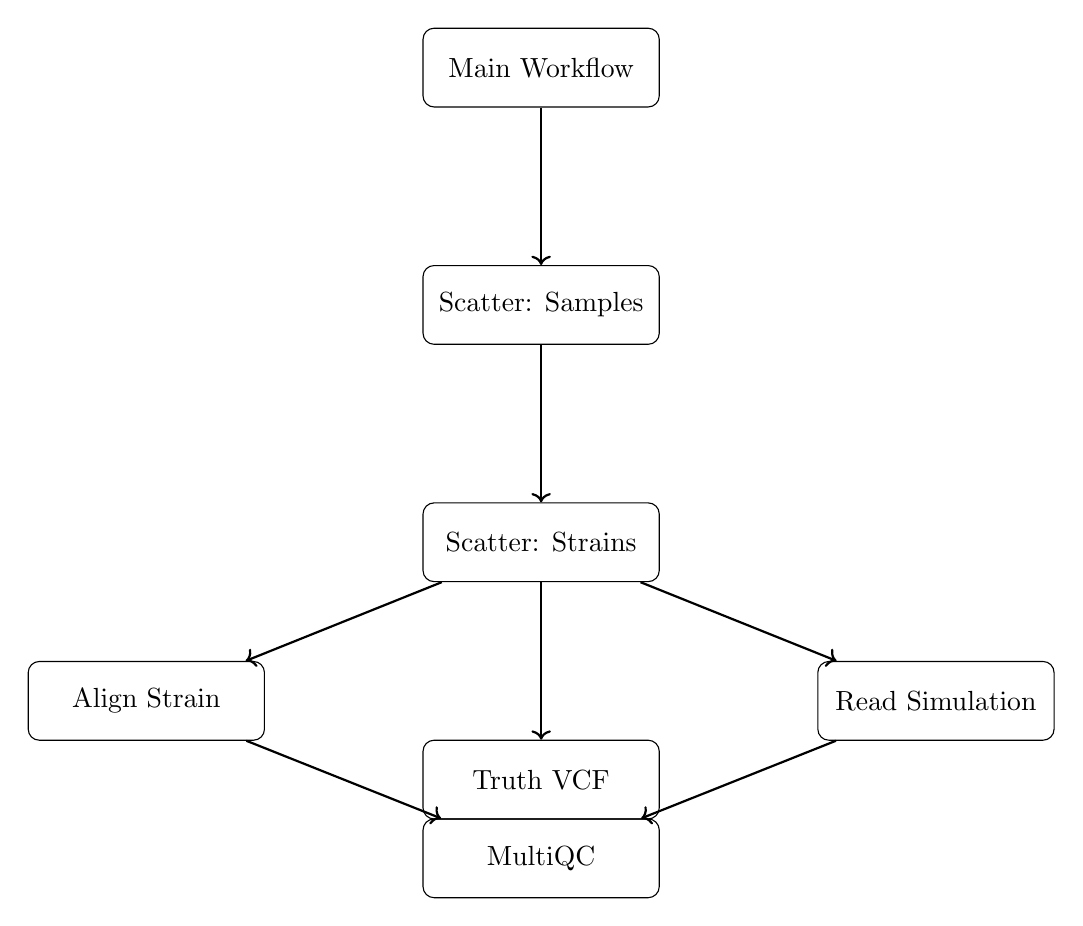
\begin{tikzpicture}[
node distance=2cm,
process/.style={rectangle, draw, rounded corners, minimum width=3cm, minimum height=1cm},
arrow/.style={->, thick}
]

\node[process] (workflow) {Main Workflow};

\node[process, below=of workflow] (samples) {Scatter: Samples};

\node[process, below=of samples] (strains) {Scatter: Strains};

\node[process, below left=1cm and 2cm of strains] (align) {Align Strain};

\node[process, below=of strains] (truth) {Truth VCF};

\node[process, below right=1cm and 2cm of strains] (simulate) {Read Simulation};

\node[process, below=3cm of strains] (multiqc) {MultiQC};

\draw[arrow] (workflow) -- (samples);
\draw[arrow] (samples) -- (strains);
\draw[arrow] (strains) -- (align);
\draw[arrow] (strains) -- (truth);
\draw[arrow] (strains) -- (simulate);
\draw[arrow] (align) -- (multiqc);
\draw[arrow] (simulate) -- (multiqc);

\end{tikzpicture}
\end{center}

\section{Pipeline Description}

\subsection{Reference Indexing}

The SARS-CoV-2 reference genome is indexed using Minimap2.  
This step generates a binary index file (.mmi) that accelerates sequence alignment.

\subsection{Strain Alignment}

Each strain genome is aligned to the reference genome using Minimap2.  
This produces SAM alignment files describing sequence differences relative to the reference.

\subsection{SAM to BAM Conversion}

SAM alignment files are converted to BAM format using Samtools.

\subsection{BAM Sorting and Indexing}

BAM files are sorted and indexed to support efficient downstream analysis.

\subsection{Ground Truth Variant Generation}

Variants between each strain genome and the reference genome are identified.  
These variant calls represent the ground truth mutations present in each strain.

\subsection{RNA Fragmentation Simulation}

Wastewater samples contain degraded RNA molecules.  
To model this phenomenon, viral genomes are fragmented into smaller segments before sequencing simulation.

Fragment lengths are drawn from a configurable distribution.

\subsection{Primer Dropout Simulation}

Primer dropout events are simulated using a BED file describing primer locations.

Selected primer regions are removed from the simulated genome fragments to mimic failed amplification.

The workflow supports samples with zero or multiple dropout regions.

\subsection{Sequencing Read Simulation}

Sequencing reads are simulated from the fragmented viral genomes according to:

\begin{itemize}
\item strain abundance
\item sequencing coverage
\item fragment size distribution
\end{itemize}

The output consists of paired-end FASTQ files.

\subsection{Multi-Sample Simulation}

The pipeline supports simulation of multiple wastewater samples simultaneously.

Each sample may have different:

\begin{itemize}
\item strain mixtures
\item primer dropout patterns
\item sequencing depth
\end{itemize}

Parallelization is implemented using WDL scatter blocks.

\subsection{Quality Control Reporting}

Quality control metrics from the simulation are aggregated using MultiQC.

The final output is an interactive HTML report summarizing sequencing statistics.

\section{Inputs}

Key workflow inputs include:

\begin{longtable}{|l|l|}
\hline
Parameter & Description \\
\hline
baseline\_fasta & SARS-CoV-2 reference genome \\
sars\_fastas & Array of strain genomes \\
sars\_strain\_names & Strain identifiers \\
strain\_fractions & Relative strain abundance \\
primer\_bed & Primer BED file \\
dropout\_tiles & Primer dropout regions \\
num\_samples & Number of simulated samples \\
coverage & Sequencing depth \\
\hline
\end{longtable}

\section{Outputs}

\begin{itemize}
\item Simulated FASTQ files
\item BAM alignment files
\item Ground truth VCF files
\item Truth metadata describing strain mixtures
\item MultiQC quality control report
\end{itemize}

\section{Running the Pipeline}

Example command using Cromwell:

\begin{verbatim}
java -jar cromwell.jar run simulate_wastewater.wdl \
     --inputs inputs.json
\end{verbatim}

\section{Version Control}

The workflow and SOP should be version controlled within the project repository.

\end{document}
